\documentclass{beamer}
%\mode<presentation>
\usepackage[utf8]{inputenc}
\usepackage[english]{babel}
\usetheme{CambridgeUS}
\usecolortheme{dolphin}
\usepackage{amsmath,amssymb,amsfonts, bm}
\usepackage{mathpazo}
\usepackage{graphicx,tabularx,epsfig}
\usepackage[compatibility=false]{caption}
\usepackage{subcaption}
\usepackage{rotating}
\usepackage{mathtools}


\setbeamertemplate{background}{\tikz[overlay,remember picture]\node[opacity=0.07]at (current page.center){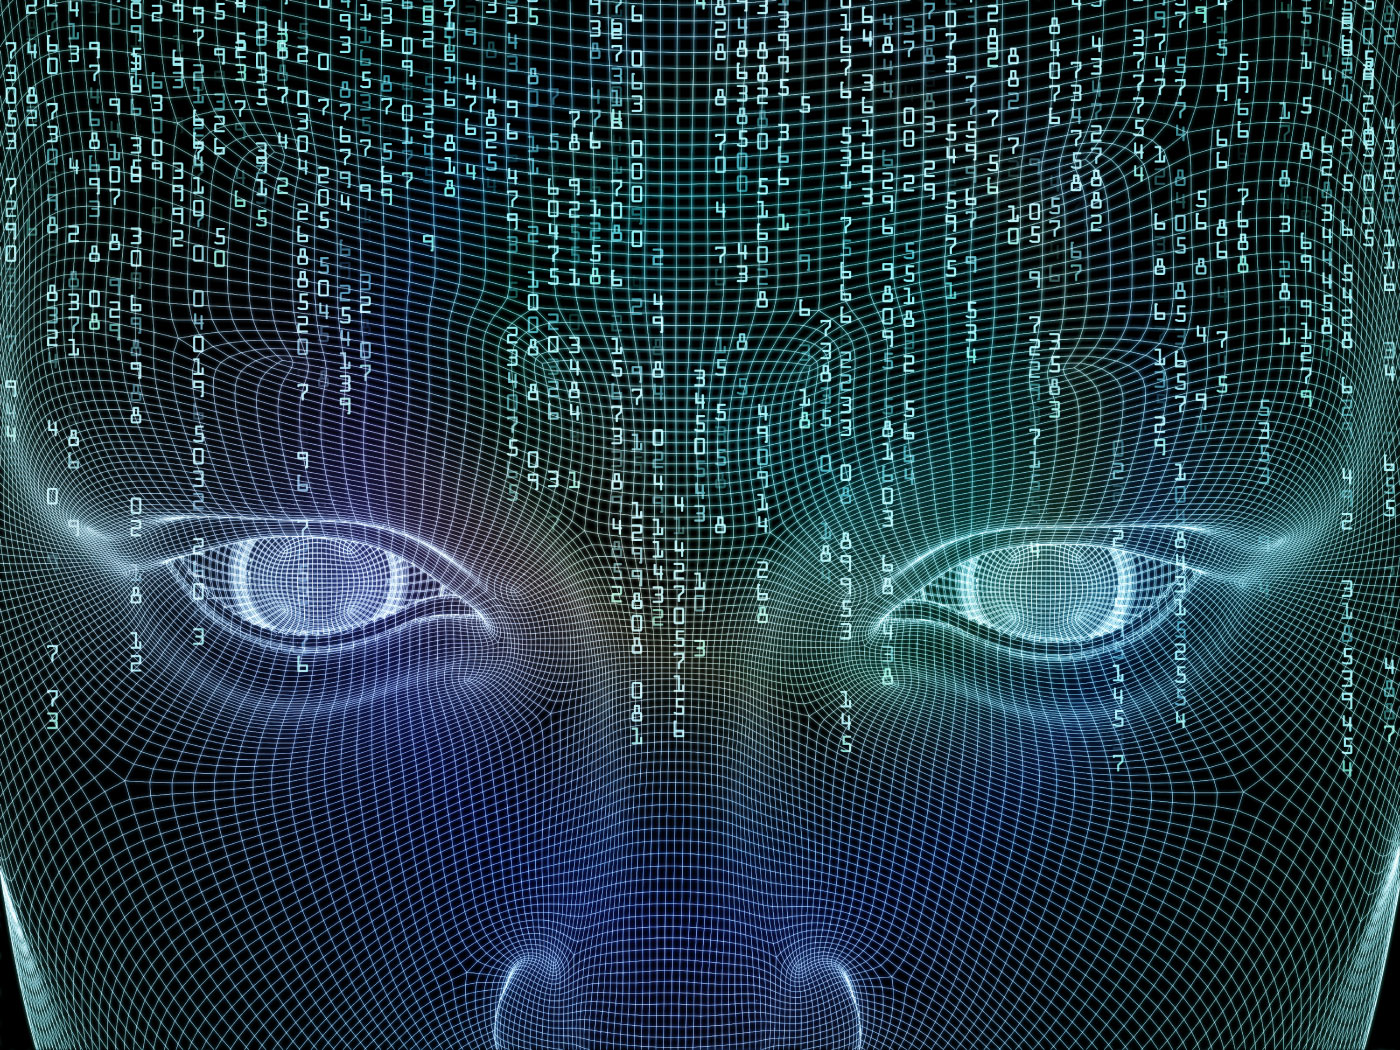
\includegraphics[width=\paperwidth]{pic/bkg}};}
\usepackage{tikz}

\DeclareGraphicsExtensions{.pdf,.png,.jpg,.svg}


\setbeamertemplate{itemize items}[square]
\setbeamertemplate{enumerate items}[square]

\definecolor{Red}{RGB}{190,0,0}
\definecolor{Blue}{RGB}{0,0,190}
\setbeamertemplate{headline}{}



\title[HBT]{PHENIX results on three-particle Bose-Einstein correlations
in $\sqrt{s_{NN}}=200$ GeV Au+Au collisions}
\author[Attila Bagoly]{\Large{Attila Bagoly for the PHENIX Collaboration
}\\ \vspace{0.1cm}}
\date[\today]{\today}
\institute[ELTE]{
}

\begin{document}

\begin{frame}
  \titlepage
\end{frame}

\begin{frame}
\frametitle{Outline}
\begin{itemize}
\setlength{\itemsep}{14pt}
\item Introduction to three-particle Bose-Einstein correlations
\item Model and fit
\item Fit results
\item Physical Interpretations
\item Summary
\end{itemize}
\end{frame}

\begin{frame}
\frametitle{Three-particle Bose-Einstein correlation function}
\begin{itemize}
\setlength{\itemsep}{8pt}
\item Invariant momentum distributions: $N_1(p_i), N_2(p_1,p_2),N_3(p_1, p_2, p_3)$
\item The definition of the correlation function:
\begin{equation*}
C_n(p_1,\dots,p_n)=\frac{N_n(p_1,\dots,p_n)}{N_1(p_1)\cdots N_1(p_n)}
\end{equation*}
 for chaotic emission:
\begin{equation*}
N_n(p_1,\dots,p_n)=\int \prod_{i=1}^{n}\mathcal{S}(x_i,p_i)|\Psi_{n}(\{x_i\})|^2 d^4x_1\dots d^4x_n
\end{equation*}
\item $\mathcal{S}(x,p)$ source function (usually assumed to be Gaussian - Levy is more general)
\begin{equation}
\mathcal{S}(\bm{r}) = \frac{1}{(2\pi)^3} \int e^{i\bm{qr}}e^{-\frac{1}{2}|\bm{r}R|^\alpha}d^3q
\end{equation}
\end{itemize}
\end{frame}

\begin{frame}
\frametitle{Core-Halo}
\begin{itemize}
\setlength{\itemsep}{20pt}
\item Not all particles comes from QGP freeze out
\item they also can come from decays
\item Both part contribute to source function:
\begin{equation*}
\mathcal{S}=\mathcal{S}_{\rm core}+\mathcal{S}_{\rm halo}
\end{equation*}

\item Two particle correlation:
\begin{equation*}
C_2(k_1, k_2) =  1+\lambda_2|\mathcal{S}(q)|^2
\end{equation*}
where
\begin{equation*}
\sqrt{\lambda_2} =  f_C \equiv \frac{N^c}{N^c+N^h} 
\end{equation*}
\end{itemize}
\end{frame}

\begin{frame}
\frametitle{Coherence}
\begin{itemize}
\setlength{\itemsep}{28pt}
\item If the core partially emits particles in coherent manner:
\begin{equation*}
\mathcal{S}_{\rm core}=\mathcal{S}_{\rm core}^{\rm pc}+\mathcal{S}_{\rm core}^{i}
\end{equation*}
where pc refers to partially coherent, i to incoherent

\item Two particle correlation: $C_2(k_1, k_2) =  1+\lambda_2|\mathcal{S}(q)|^2$, but $\lambda_2 \neq f_C^2$
\item Fraction of coherently produced pions:
\begin{equation*}
p_C \equiv \frac{N_{\rm coherent}}{N^{\rm coherent}+N^{\rm incoherent}} \rightarrow \lambda_2(f_C, p_C)
\end{equation*}
\end{itemize}

\end{frame}

\section{Motivation}
\begin{frame}
\frametitle{Motivation behind three particle HBT analysis}
\begin{itemize}
\setlength{\itemsep}{20pt}
\item $n$-particle correlation strength: $\lambda_n \equiv C_n(0)-1$
\item Core-Halo: \vspace*{-15pt}
	\begin{align*}
		\lambda_2=f_C^2,\;\;\;\;\lambda_3 = 2f_C^3+3f_C^2 \\ 
		\kappa_3=\big(\lambda_3-3\lambda_2\big)/\big(2\sqrt{\lambda_2^3}\big)=1
	\end{align*}
\item Partial coherence ($p_C$ fraction of coherently produced $\pi$): 
	\begin{gather*}
		\lambda_2=f_C^2\big[(1-p_C)^2+2p_C(1-p_C)\big]\\
		\lambda_3=2f_C^3\big[(1-p_C)^3+3p_C(1-p_C)^2\big]+3f_C^2\big[(1-p_C)^2+2p_C(1-p_C)\big]\nonumber\\
		\kappa_3 = \kappa_3(p_C)
	\end{gather*}
\item From $\lambda_2$, $\lambda_3$ we can investigate the deviation from simple Core-Halo
\end{itemize}
\end{frame}

\section{Model}
\begin{frame}
\frametitle{Model without Coulomb correction}
\begin{itemize}
\setlength{\itemsep}{22pt}

\item Correlation function ($\mathcal{L}_3=2f_C^3$):
\begin{align*}
C_3^{(0)}(k_{12}, k_{13}, k_{23}) = 1+ \ell_3e^{-0.5(|2k_{12}R_C|^\alpha+|2k_{13}R_C|^\alpha+|2k_{23}R_C|^\alpha)}\nonumber\\
+\ell_2\bigg(e^{|2k_{12}R_C|^\alpha}+e^{|2k_{13}R_C|^\alpha}+e^{|2k_{23}R_C|^\alpha}\bigg)
\end{align*}
\item Background: $N(1+\epsilon k_{12})(1+\epsilon k_{13})(1+\epsilon k_{23})$
\item Fit parameters: $\ell_3$, $\ell_2$,  $R_C$, $\alpha$, $N$, $\epsilon$
\item We are looking for: $\lambda_3 \equiv  C_3(k_{12}=k_{13}=k_{23}=0)-1=\ell_3+3\ell_2$
\end{itemize}
\end{frame}

\begin{frame}
\frametitle{Coulomb correction}
\begin{itemize}
\setlength{\itemsep}{16pt}
\item Corrected model:
\begin{equation*}
C_3(k_{12}, k_{13}, k_{23}) = C_3^{(0)}(k_{12}, k_{13}, k_{23})\cdot K_3(k_{12}, k_{13}, k_{23})
\end{equation*}
\item ''Generalized Riverside'' method for 3 particle Coulomb problem
\begin{equation*}
K_3(k_{12}, k_{13}, k_{23}) \approx K_1(k_{12})K_1(k_{13})K_1(k_{23})
\end{equation*}
\end{itemize}
\begin{figure}
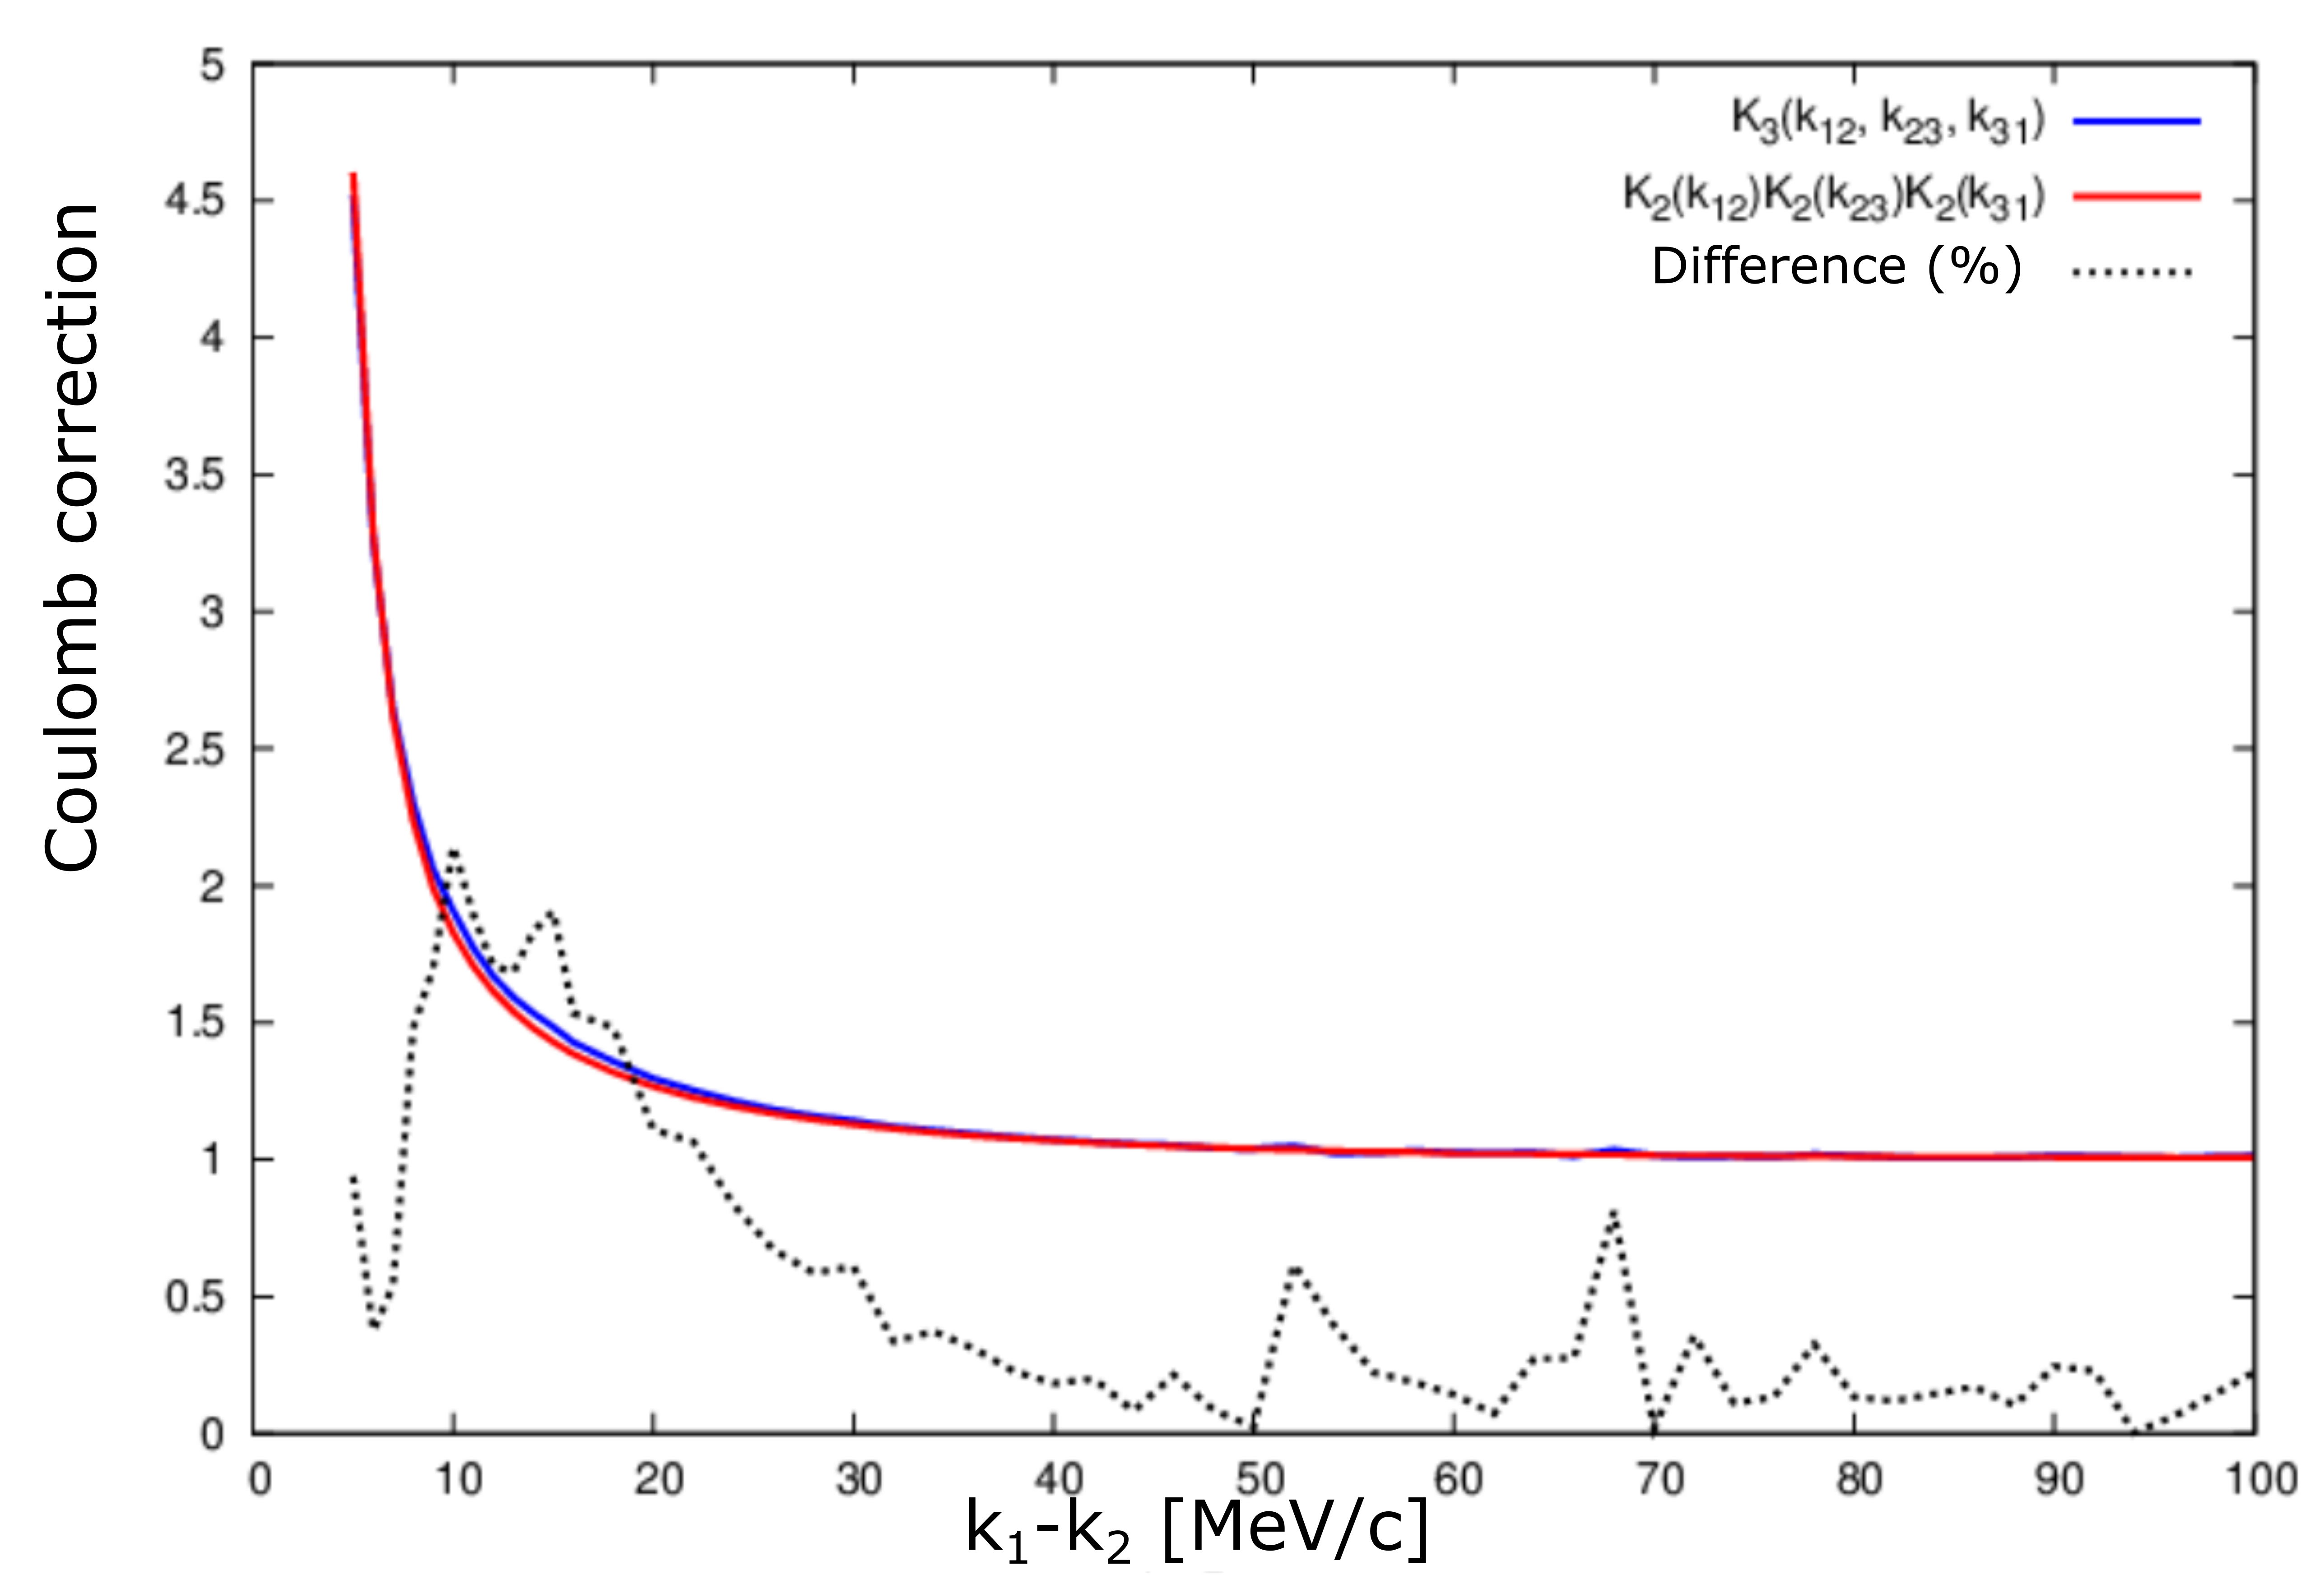
\includegraphics[scale=0.25]{pic/coulomb1}
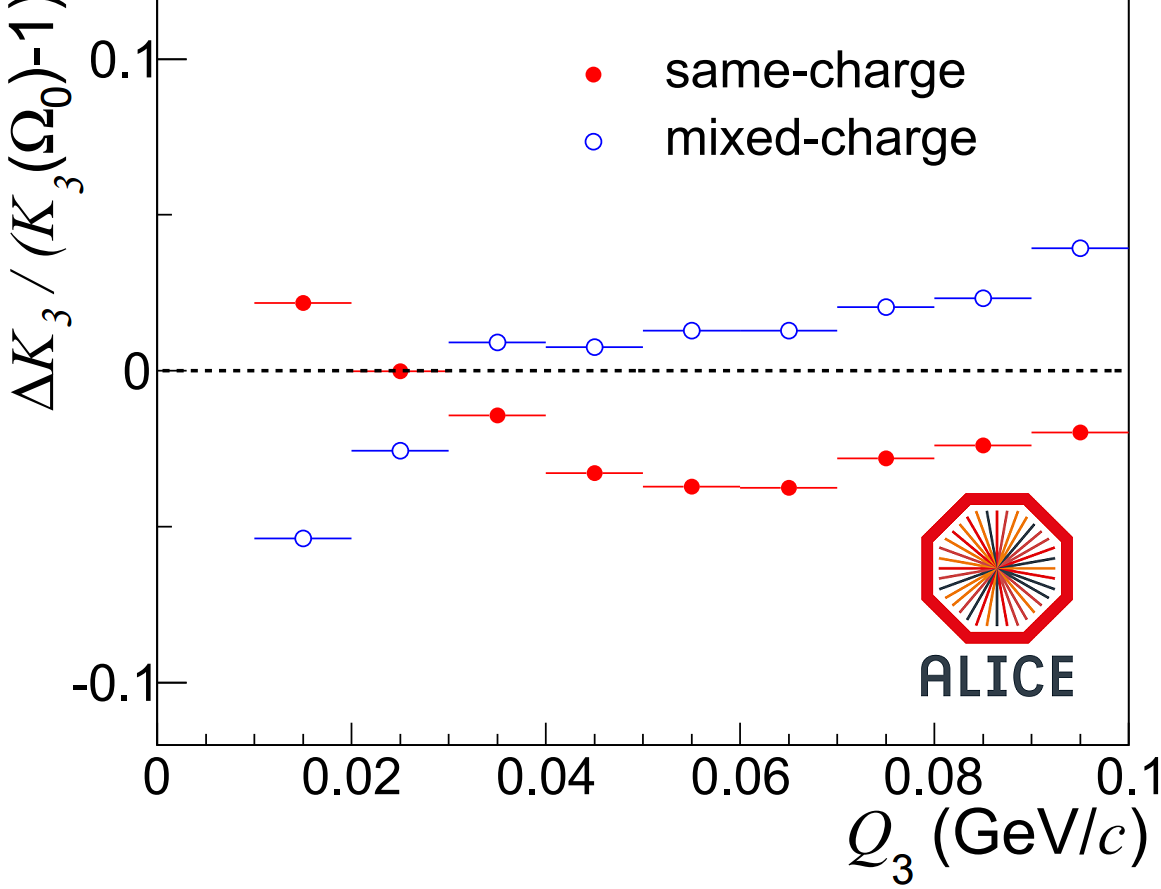
\includegraphics[scale=0.235]{pic/coulomb2}
\end{figure}
\end{frame}


\begin{frame}
\frametitle{Diagonal visualization of fits}
\begin{itemize}
\setlength{\itemsep}{16pt}
\item Visualization in $k_{12}=k_{23}=k_{13}$ subspace: shows good fits
\end{itemize}
\begin{figure}
\hspace*{-0.5cm}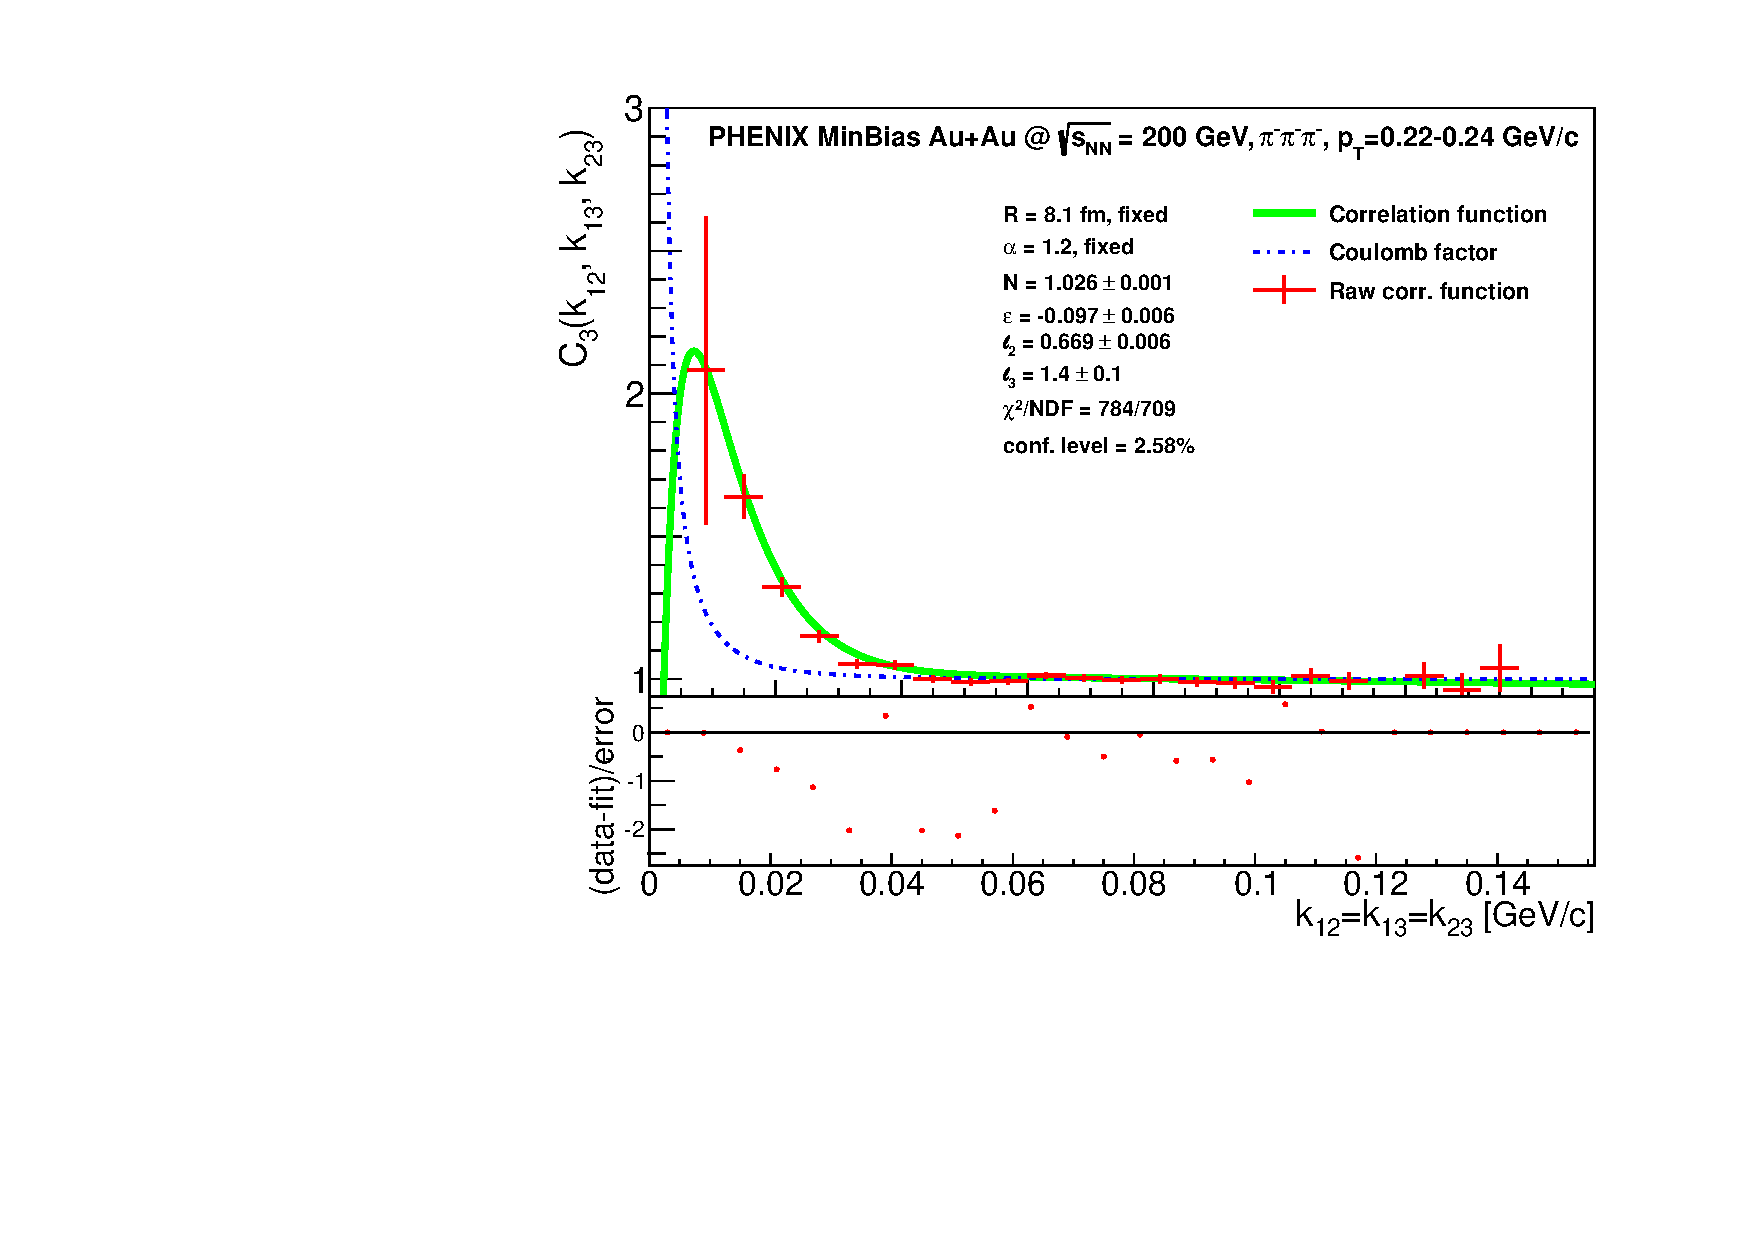
\includegraphics[scale=0.35]{pic/diag_lowpt.pdf}
 \hspace*{-0.6cm}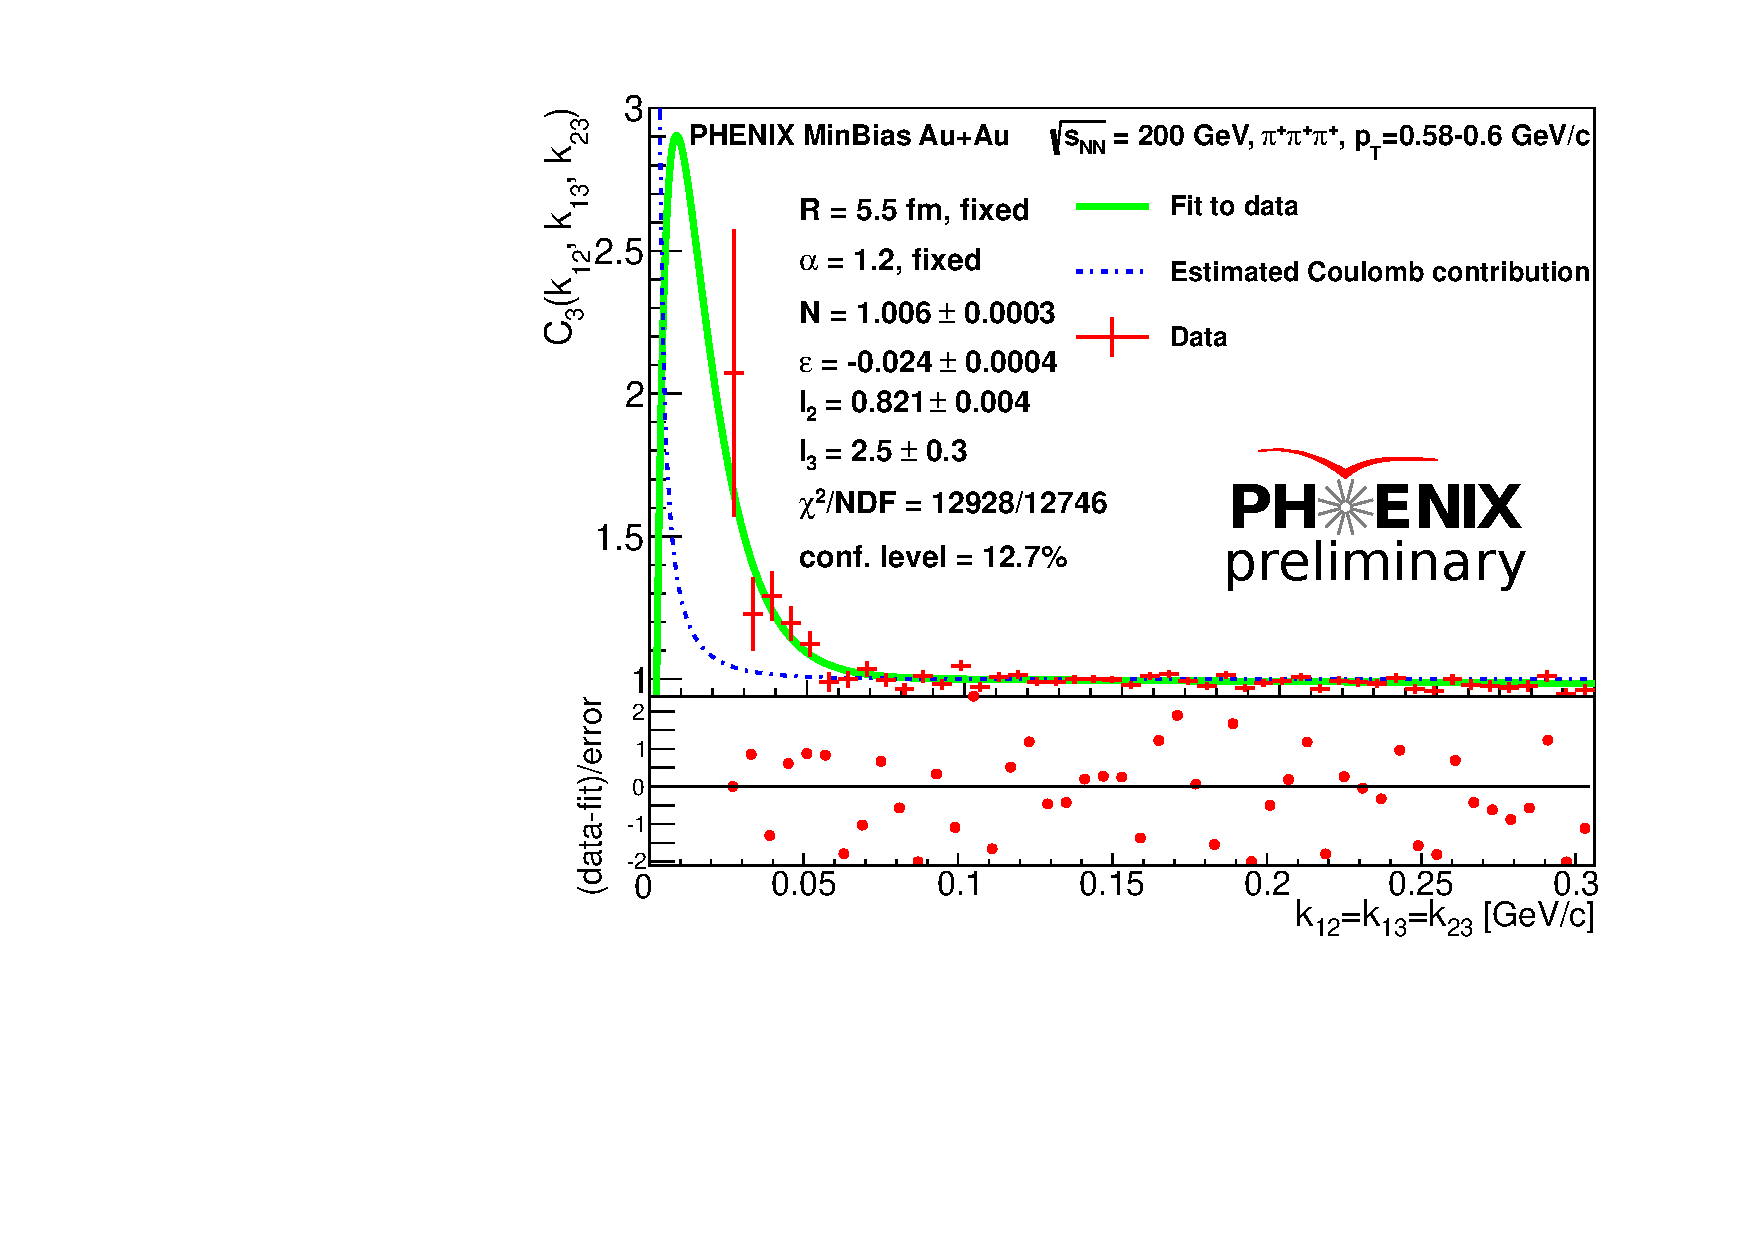
\includegraphics[scale=0.35]{pic/diag_highpt.pdf}
\end{figure}
\end{frame}


\begin{frame}
\frametitle{Three particle correlation strength: $\lambda_3$}
\begin{itemize}
\setlength{\itemsep}{10pt}
\item $\lambda_3$ within Core-Halo  + chaotic emission range for all $m_T$
\end{itemize}
\begin{figure}
\colorbox{white}{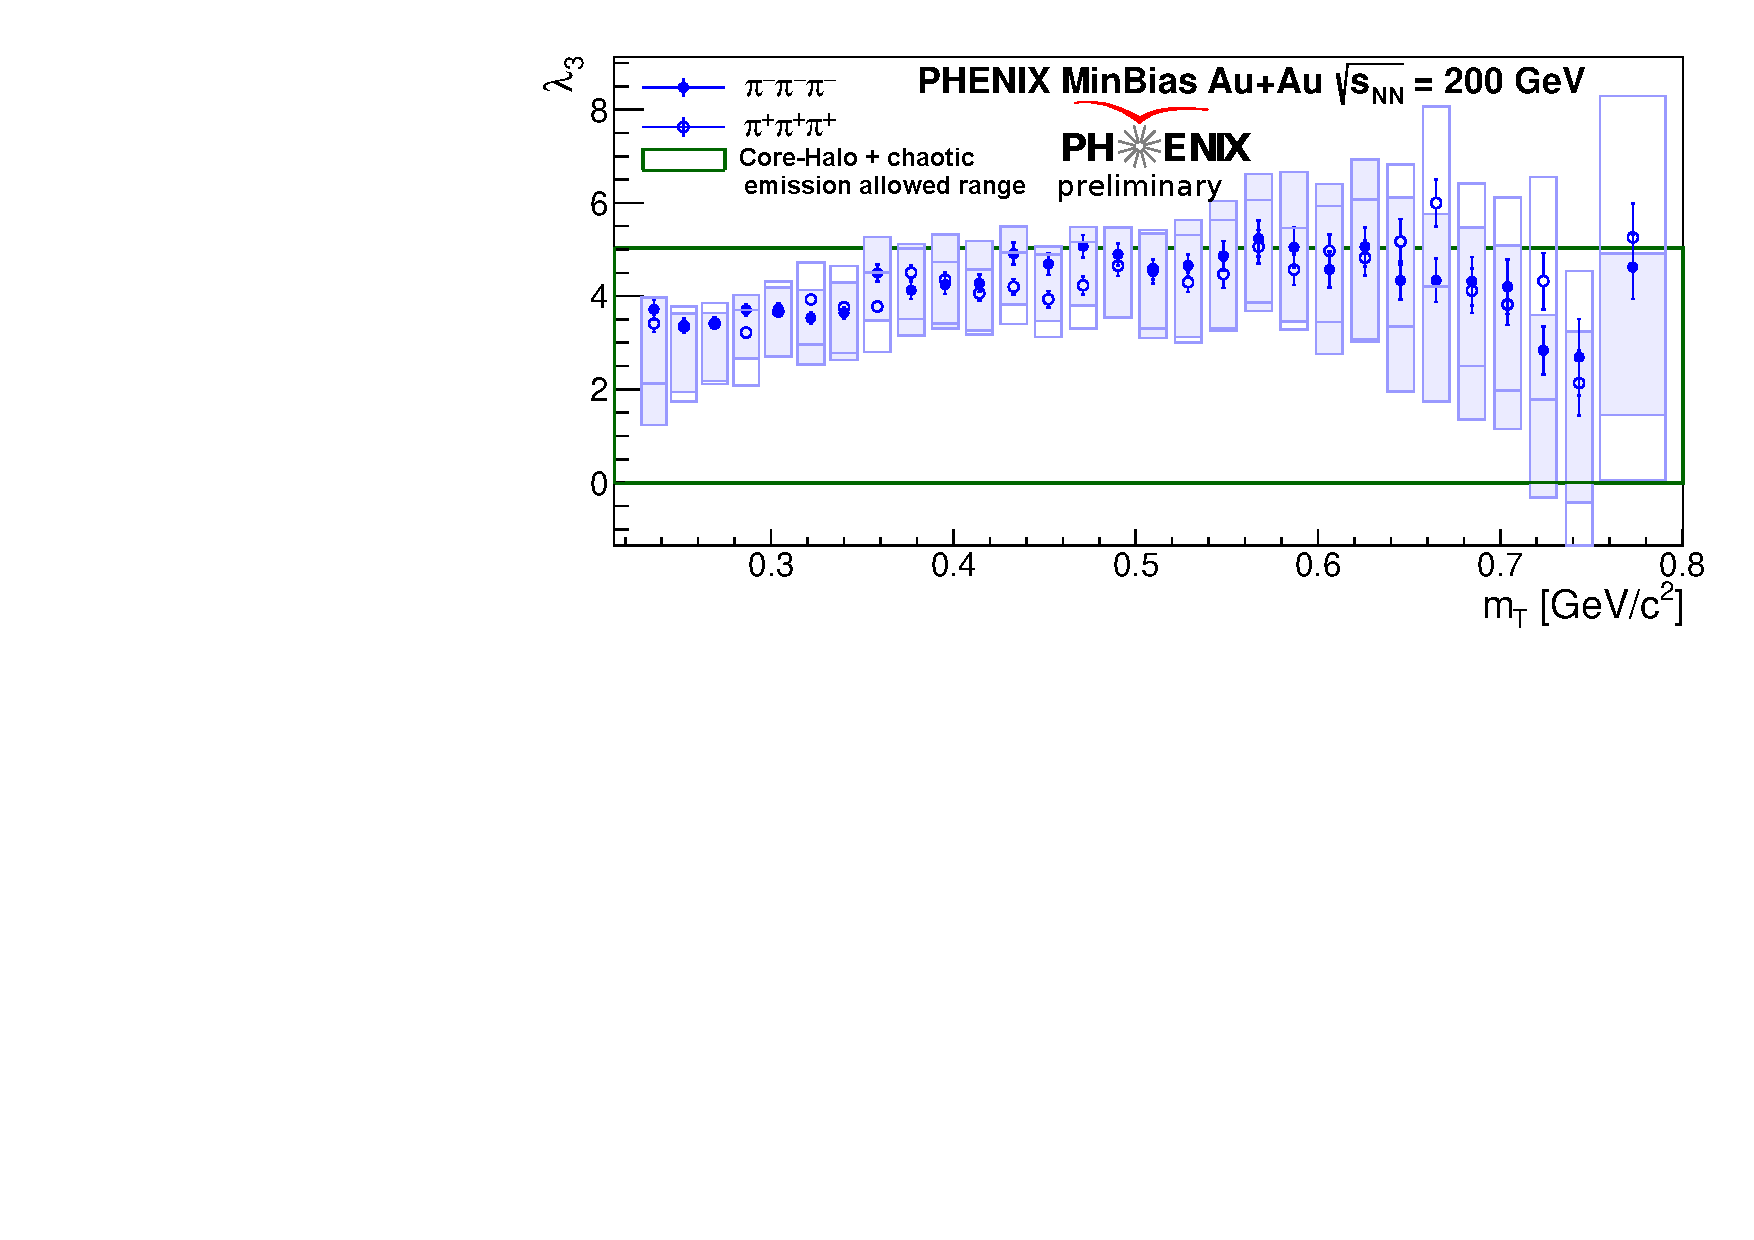
\includegraphics[scale=0.6]{pic/lambda3}}
\end{figure}
\end{frame}



\begin{frame}
\frametitle{Core-Halo independent parameter}
\begin{itemize}
\item $\kappa_3\equiv\frac{\lambda_3-3\lambda_2}{2\sqrt{\lambda_2^3}}$ not depend on $f_C$ ($f_C=\mathrm{core}/(\mathrm{core}+\mathrm{halo})$)
\item Core-Halo + chaotic emission: $\kappa_3=1$
\item additional effect (eg. not fully thermal): $\kappa_3\neq 1$
\item Statistically significant deviation from $\kappa_3=1$
\end{itemize}
\begin{figure}
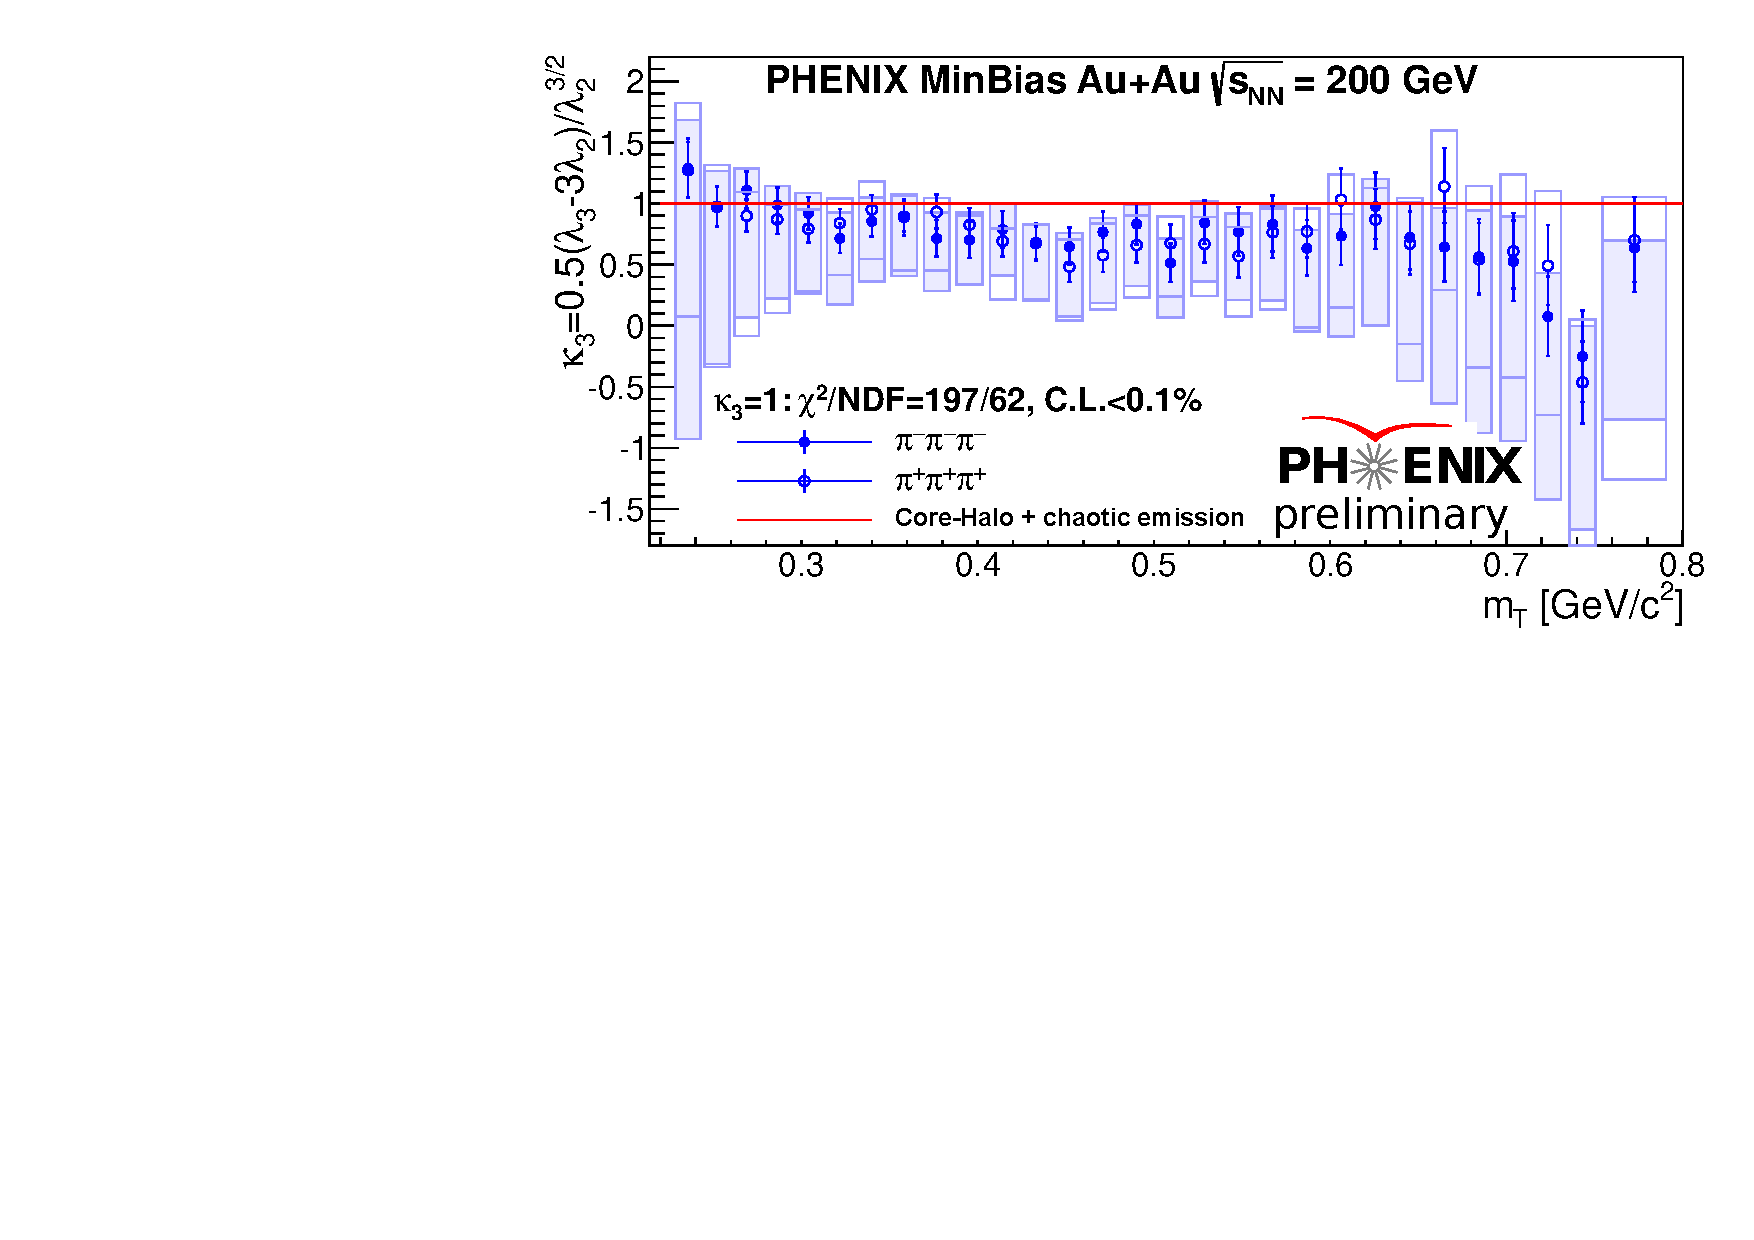
\includegraphics[scale=0.5]{pic/kappa3}
\end{figure}
\end{frame}


\begin{frame}
\frametitle{Partial coherence ($p_c$) vs fractional core}
\begin{itemize}
\vspace{-0.004\textheight}
\item Simple theoretical model: $\lambda_2(f_c, p_c)$, $\lambda_3(f_c, p_c)$ 
\item Measured $\lambda_2^{\rm meas.} \rightarrow \lambda_2^{\rm meas.}=\lambda_2(f_c,p_c) \Longrightarrow f_c(p_c)$ (green lines)
\item Measured $\lambda_3^{\rm meas.} \rightarrow \lambda_3^{\rm meas.}=\lambda_3(f_c,p_c) \Longrightarrow f_c(p_c)$ (blue lines)
\item $f_c<0.82$ and $p_c>0.5$ can be excluded, $p_C<0.5$ can't be excluded
\end{itemize}

\begin{figure}
\hspace*{-0.29cm}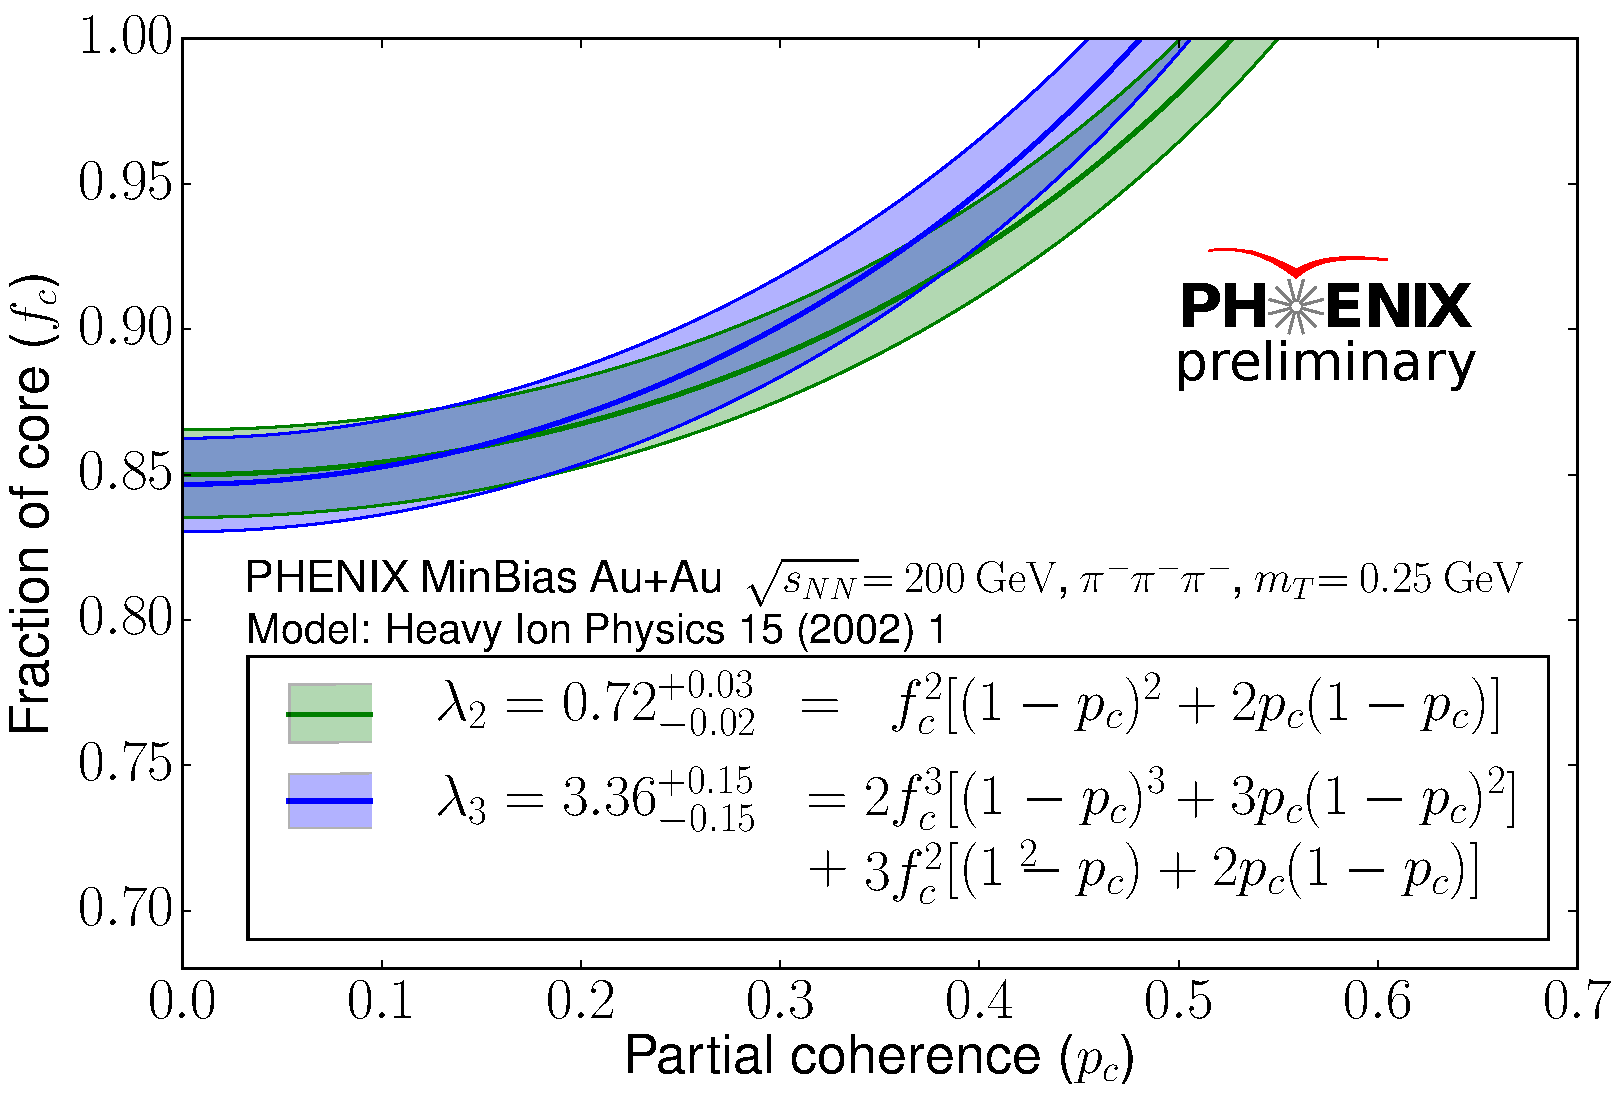
\includegraphics[width=0.53\textwidth]{pic/cropped_fcpc1}
\hspace*{-0.05cm}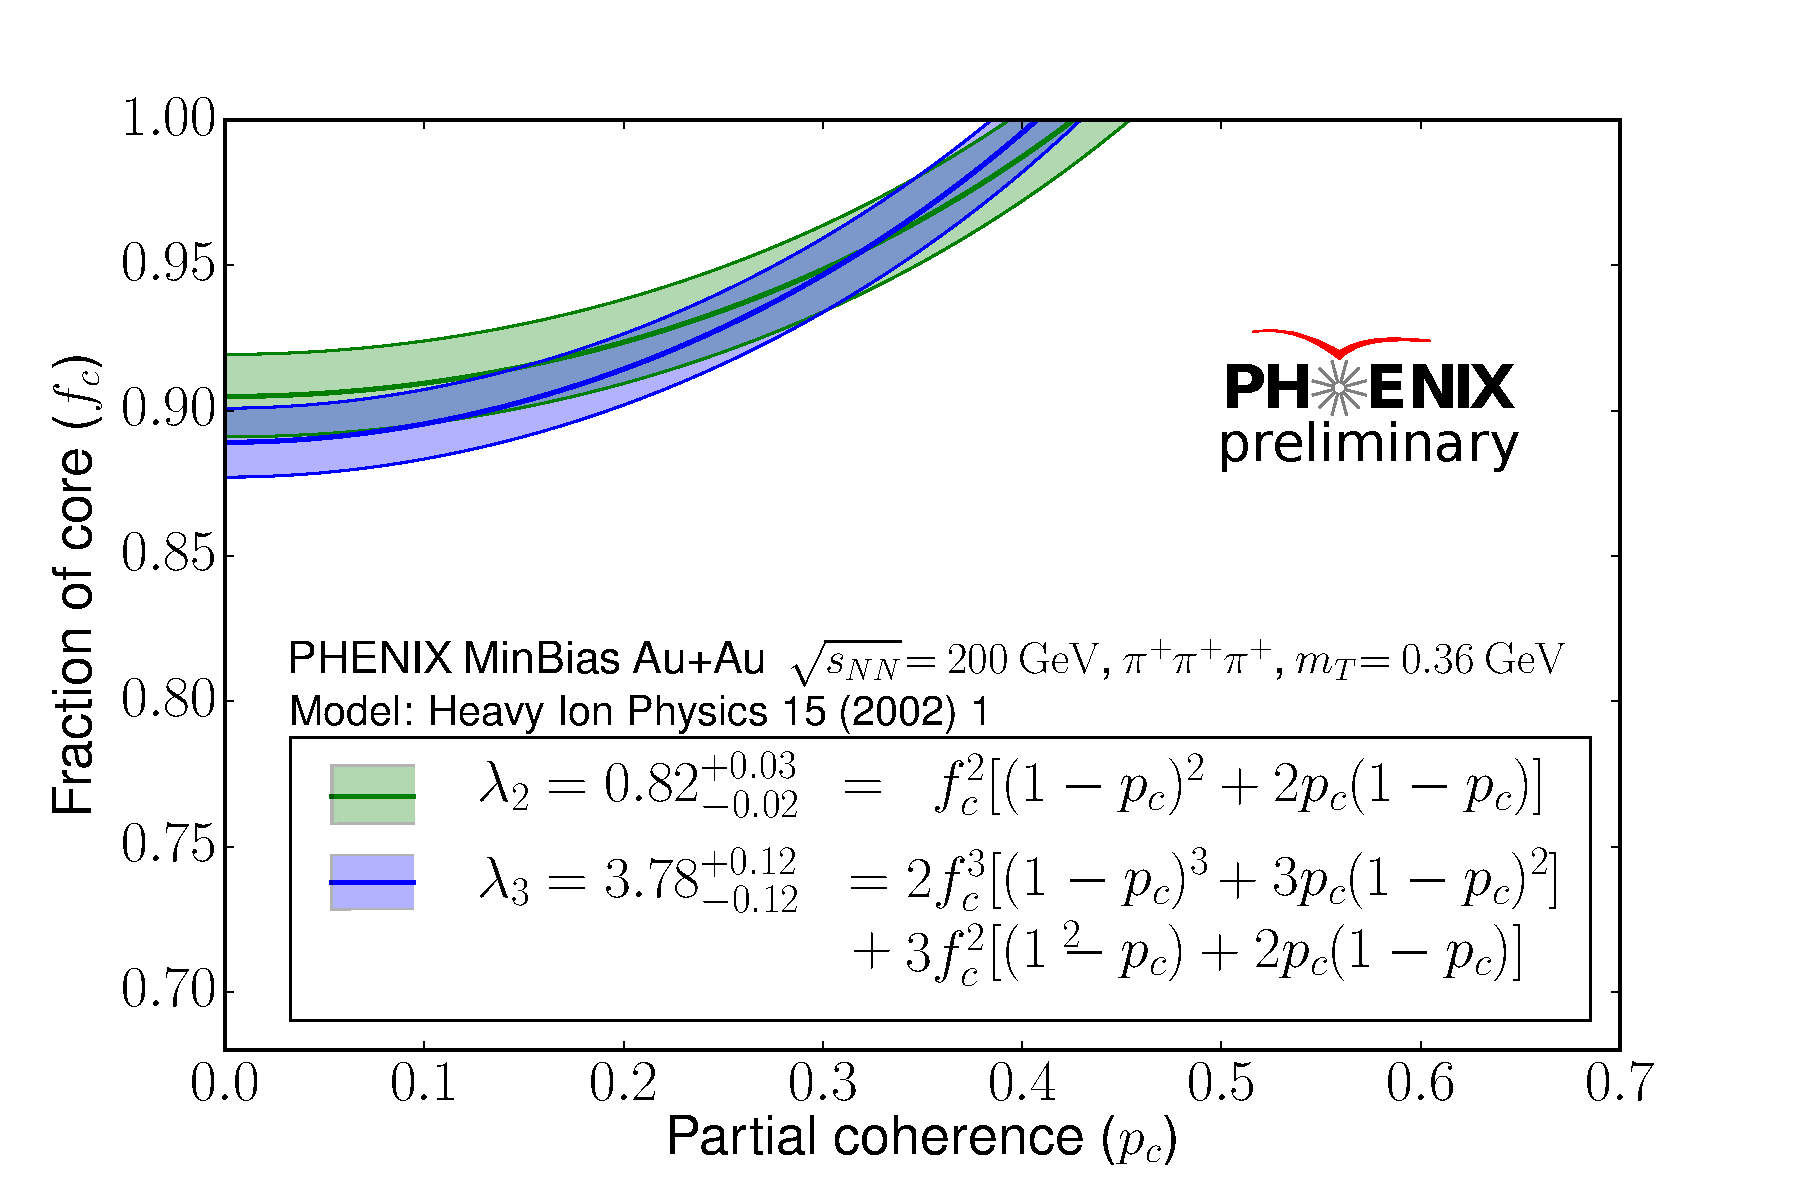
\includegraphics[width=0.53\textwidth]{pic/cropped_fcpc2}
\end{figure}
\end{frame}

\begin{frame}
\frametitle{Summary}
\begin{itemize}
\setlength{\itemsep}{14pt}
\item Three-pion BE correlation functions from 200 GeV Au+Au data
\item Lévy-distribution for describing the source
\item Measured $\lambda_3$ correlation strength within Core-Halo + chaotic emission limit
\item PHENIX preliminary $\kappa_3$ data shows a significant effect
\item $\lambda_2$ and $\lambda_3$ analysis: possibility for partial coherence
\item We need to:
\begin{itemize}
\item finalize this analysis for $0-30\%$
\item study detailed centrality and $\sqrt{s_{NN}}$ dependence
\end{itemize}
\end{itemize}
\end{frame}


\end{document}

